\chapter{系统工作流程与实证分析}
\section{系统整合}
基于前几章的描述,我们可以综合构建一个数据挖掘系统,发现用户兴趣,推荐相关内容。
图\ref{fig:systemflow}展现了整体系统流程。

\usetikzlibrary{shapes,snakes}
\usetikzlibrary{arrows, decorations.markings}

\tikzstyle{vecArrow} = [thick, decoration={markings,mark=at position
   1 with {\arrow[semithick]{open triangle 60}}},
   double distance=1.4pt, shorten >= 5.5pt,
   preaction = {decorate},
   postaction = {draw,line width=1.4pt, white,shorten >= 4.5pt}]

% Define box and box title style
\tikzstyle{mybox} = [draw=black, fill=white, very thick,
    rectangle, rounded corners, inner sep=10pt, inner ysep=20pt]
\tikzstyle{fancytitle} =[fill=red, text=white]

\def\html{
    \draw[rounded corners=0.1ex,fill=white,thick] (0.2,0.2) rectangle (1.2,1.5);
    \draw[rounded corners=0.1ex,fill=white,thick] (0.1,0.1) rectangle (1.1,1.4);
    \draw[rounded corners=0.1ex,fill=white,thick] (0,0) rectangle (1,1.3);
    \node at (0.5,0.3) {\tiny HTML};
}

\begin{center}
\begin{tikzpicture}
\node [mybox] (stepone){
	\begin{minipage}{0.40\textwidth}
		Web Logs and HTML files
		\newline
		\tiny
        \begin{center}
		\begin{tabular}{@{} c @{}|@{} c @{}|@{} c @{}|@{} c @{}|@{} c @{}|@{} c @{}}
			\hline
			User ID & Request URL & Time & Location & Content & Device \\
			\hline
			1 & www.$\ldots$/bbb & 20:10 & hill & $\ldots$ & iPhone \\
			\hline
			2 & www.$\ldots$/aab & 23:20 & base & $\ldots$ & iPhone \\
			\hline
			3 & www.$\ldots$/cdd & 24:10 & grid & $\ldots$ & iPhone \\
			\hline
		\end{tabular}
		\end{center}
	\end{minipage}
};
\begin{scope}[xshift=50,yshift=15]
\html
\end{scope}
\draw [->] (1.5,-0.5) -- (2,1);
\node[fancytitle, right=10pt] at (stepone.north west) {网络流量信息采集};

\node[mybox, right=10pt] at (stepone.east) (steptwo){
	\begin{minipage}{0.40\textwidth}
		HTML classification
		\newline
		\tiny
        \begin{flushright}
		\begin{tabular}{@{} c @{}|@{} c @{}|@{} c @{}|@{} c @{}|@{} c @{}|@{} c @{}}
			\hline
			User ID & Request URL & Item \\
			\hline
			1 & www.$\ldots$/bbb & cat \\
			\hline
			2 & www.$\ldots$/aab & car \\
			\hline
			3 & www.$\ldots$/cdd & pig \\
			\hline
		\end{tabular}
		\end{flushright}
	\end{minipage}
};
\begin{scope}[xshift=120,yshift=-35]
\html
\end{scope}
\node[fancytitle, right=10pt] at (steptwo.north west) {语义分析及内容分类};

\draw [->] (5.4,-0.1) -- (6.2,0.1);
\draw [->] (5.3,-0.4) -- (6.2,-0.4);
\draw [->] (5.2,-0.7) -- (6.2,-1);
\node [draw] at (6.5,0.1) {\footnotesize cat};
\node [draw] at (6.5,-0.4) {\footnotesize car};
\node [draw] at (6.5,-1) {\footnotesize pig};

\node[mybox, below=10pt] at (stepone.south) (stepfour){
	\begin{minipage}{0.40\textwidth}
		Prediction matrix
		\newline
		\tiny
        \begin{center}
		\begin{tabular}{@{} c @{}|@{} c @{}|@{} c @{}|@{} c @{}|@{} c @{}|@{} c @{}}
			\hline
			 & Item 1 & Item 2 & Item 3 \\
			\hline
			User 1 & \textbf{0.7} & 0.8 & 0.9 \\
			\hline
			User 2 & 0.1 & 0.6 & \textbf{0.5} \\
			\hline
			User 3 & 0.2 & \textbf{0.4} & 0.3 \\
			\hline
		\end{tabular}
		\end{center}
	\end{minipage}	
};

\node[mybox, below=10pt] at (steptwo.south) (stepthree){
	\begin{minipage}{0.40\textwidth}
		User-Item matrix
		\newline
		\tiny
        \begin{center}
		\begin{tabular}{@{} c @{}|@{} c @{}|@{} c @{}|@{} c @{}|@{} c @{}|@{} c @{}}
			\hline
			 & Item 1 & Item 2 & Item 3 \\
			\hline
			User 1 & ? & 0.8 & 0.9 \\
			\hline
			User 2 & 0.1 & 0.6 & ? \\
			\hline
			User 3 & 0.2 & ? & 0.3 \\
			\hline
		\end{tabular}
		\end{center}
	\end{minipage}
};
\node[fancytitle, right=10pt] at (stepfour.north west) {协同过滤预测};
\node[fancytitle, right=10pt] at (stepthree.north west) {数据格式预处理};

\draw[vecArrow] (stepone) to (steptwo);
\draw[vecArrow] (steptwo) to (stepthree);
\draw[vecArrow] (stepthree) to (stepfour);
\end{tikzpicture}
\figurecaption{整体系统流程}
\label{fig:systemflow}
\end{center}
\begin{center}
\def\sysleft{
    \node at (0,0) [rectangle,draw] {Data from \textbf{Feb}};
    \node at (0,1) [rectangle,draw] {Data from \textbf{Jan}};
    \node at (0,2) [rectangle,draw] {Data from \textbf{Dec}};
    \node at (0,5) [rectangle,draw] {Data from \textbf{Nov}};
    \node at (0,3) [align=center] {\textbf{Data proccessing}\\
             \textbf{in Recommend system}};
    \draw (-2.2,-1) rectangle (2.2,4);
}
\def\sysright{
    \node at (0,0) [rectangle,draw] {Data from \textbf{Mar}};
    \node at (0,1) [rectangle,draw] {Data from \textbf{Feb}};
    \node at (0,2) [rectangle,draw] {Data from \textbf{Jan}};
    \node at (0,5) [rectangle,draw] {Data from \textbf{Dec}};
    \node at (0,3) [align=center] {\textbf{Data proccessing}\\
             \textbf{in Recommend system}};
    \draw (-2.2,-1) rectangle (2.2,4);
}
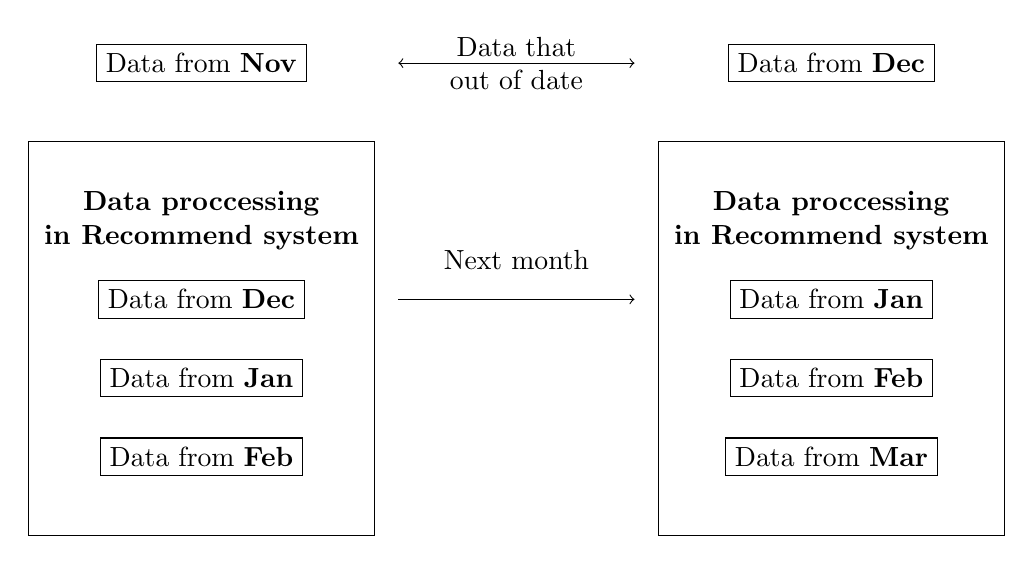
\begin{tikzpicture}
\sysleft
\begin{scope}[xshift=8cm]
\sysright
\end{scope}
\draw[->] (2.5,2) -- (5.5,2);
\node at (4,2.5) {Next month};
\node at (4,5) [align=center] {Data that\\
                                    out of date};
\draw[<->] (2.5,5) -- (5.5,5);
\end{tikzpicture}
\figurecaption{推荐系统数据的流动性}
\label{fig:dataflow}
\end{center}

本文构建的推荐系统将按照图\ref{fig:systemflow}中的箭头指向运行。
但是在现实情况中,社会的信息是流通的,新的事物会不断出现,而人们的兴趣也会不断地改变。
所以推荐系统的运行过程不是一次性的。
推荐系统所使用的用户数据应该具有流的形式,即在推荐的过程中获取新的用户数据,并丢弃旧的数据。

如图\ref{fig:dataflow},在3月份时,处理的是12月、1月、2月的数据,为3月的应用访问做推荐;到4月份时,处理的是1月、2月、3月的数据,12月份的数据被丢弃。
或者采取加权的形式,比如最近一个月的数据权重较高,其它历史月份的权重较低。

下面将根据整体系统流程图,简单介绍真实数据测试的方法、流程及结果。

\section{真实数据测试}
本文采用的测试硬件主要包括4台安装了64位Ubuntu14.04以及Hadoop2.6.4的服务器,其配置包含2个Intel的Xeon的CPU,型号为E5-2630,核心频率2.30GHz,2GB内存,40GB硬盘空间,其中一台服务器作为Master,另外三台服务器作为Slave。

由于测试数据的限制,本文无法对系统整体测试,只能按照各模块的功能进行测试。
在图\ref{fig:systemflow}中,关键步骤为第二步语义分析及内容分类以及第四步协同过滤预测。
在语义分析及内容分类步骤中,本文采用了精确度较高的ICTCLAS中文分词系统\parencite{Zhang2003CLA}。
ICTCLAS中文分词系统的各项测试数据在其下载页面已有详细介绍,本文不再重复。

在协同过滤预测步骤中,采用了4个不同的数据集,分别是:
MovieLens的144MB的数据集,其中包含了截止到2016年1月,240000多位用户对33000多部电影的22000000个评分数据,以及58000000个类型标记;
2015年阿里移动推荐算法比赛的129MB的数据集,其中包含2014年11月12日到2014年12月11日间,10000多名用户在淘宝线上与1900000多个商品的互动信息,即浏览、收藏、加入购物车以及购买等动作;
雅虎音乐1.5GB的C15数据集,其中包括2002年到2006年间,18223179位雅虎用户对136736首歌的717872016个评分;另外还有雅虎音乐1.6GB的R2数据集,其中包含用户对音乐、歌手、专辑的评分,数据量级与C15数据集相似。

在4个数据集中,阿里移动推荐算法比赛的数据集,相对而言,是最满足本推荐模块测试要求的。
因为用户与商品的互动信息,是二值信息,即有没有发生过该类互动。
而互联网用户在浏览网页中,表现对某关键字兴趣爱好也是二值信息,即感兴趣,或者不感兴趣。
当然,也可以将该二值信息改为类似评分值的连续值,即按浏览该网页时间,点击该网页等计算出兴趣爱好值。

在测试基于交互历史的协同过滤推荐系统时,要将数据集分为训练集以及测试集。
训练集用于训练协同过滤推荐系统中的参数,测试集用于计算推荐的优良程度。
由于数据集中的评分记录都有时间戳,所以可以按时间区分训练集与测试集。
本文采用,评分记录按时间排序后,前80\%的记录作为训练集,后20\%的记录作为测试集的区分方案。

推荐系统的优良程度可以采取F1分数来评价。此时F1分数的定义如下:
\begin{center}
\begin{itemize}
	\item $PredictionSet$:预测评分大于最大评分一半的记录组成的集合
	\item $ReferenceSet$:测试集中评分大于最大评分一半的记录组成的集合
\end{itemize}
\end{center}
此时再定义精确度$precision$与召回率$recall$如下:
\begin{equation}
precision= \frac{|PredictionSet\cap ReferenceSet|}{|PredictionSet|}
\end{equation}
\begin{equation}
recall= \frac{|PredictionSet\cap ReferenceSet|}{|ReferenceSet|}
\end{equation}
则F1分数为
\begin{equation}
F= 2* \frac{precision*recall}{precision+recall}
\end{equation}

表\ref{table:performance}展示了协同过滤推荐系统在四个数据集中的F1分数。
其中F1分数稳定在0.07的范围,表明协同过滤推荐系统在F1分数这种评价标准中表现并不太好。
造成这个结果的主要原因是,F1分数比较适用于评价二分类问题。
而协同过滤算法计算得到的实数值对二分类问题的界定线比较敏感。
\begin{center}
\tablecaption{协同过滤推荐系统的性能分析}
\label{table:performance}
\begin{tabular}{c|c|c}
 \hline
数据集 & 训练集大小 & F1 score \\ \hline
MovieLens & 576MB & 0.0823 \\ \hline
Aliyun contest & 516 & 0.0644 \\ \hline
Yahoo! R2 & 6.4GB & 0.0876 \\ \hline
Yahoo! C15 & 6.0GB & 0.0713 \\ \hline
\end{tabular}
\end{center}
\pgfplotsset{compat=1.13}
\begin{center}
\begin{tikzpicture}
\begin{axis}[
    ybar,
    enlargelimits=0.15,
    legend style={at={(0.5,-0.2)},
      anchor=north,legend columns=-1},
    ylabel={每个map阶段平均运行时间(s)},
    xlabel={特征空间维数$r$},
    symbolic x coords={U10,M10,U20,M20,U50,M50,U100,M100},
    xtick=data,
    nodes near coords,
    nodes near coords align={vertical},
    x tick label style={rotate=45,anchor=east},
    ]
    \addplot coordinates {(U10,42) (M10,43) (U20,41) (M20,42)
         (U50,35)(M50,48) (U100,37)(M100,60)};
    \addplot coordinates {(U10,46) (M10,52) (U20,44) (M20,59)
         (U50,52)(M50,96) (U100,87)(M100,161)};
	 \legend{MovieLens,Yahoo! C15}
\end{axis}
\end{tikzpicture}
\figurecaption{基于模型的协同过滤推荐系统的测试}
\label{fig:MCFtest}
\end{center}

图\ref{fig:MCFtest}是对基于模型的协同过滤推荐系统测试。
在该测试中,我们使用了MovieLens和雅虎音乐C15两个数据。
对于MovieLens数据,无论特征空间维数$r$多大,每个map阶段的平均运行时间落在35秒到60秒的区间。
这表明,对于小的数据集,其运行时间主要由Hadoop自身的工作调度决定。
对于比较大的雅虎音乐数据,我们可以发现特征空间维数$r$较小时,其运行时间主要由Hadoop自身的工作调度决定。
但是当特征空间维数$r$较大时,其运行时间主要由分发、计算特征矩阵过程决定。
另外,我们还注意到,计算物品特征矩阵$M$用时比计算用户特征矩阵$U$用时更多,这是因为用户集$U$
中用户数目大概是物品集$M$的20倍,所以要花更多时间来分发矩阵$U$。
实验表明,对于MovieLens数据,每小时能计算37到47次迭代。而对于雅虎音乐C15数据,每小时能计算15到38次迭代。
这表明对于包含百万级交互信息的数据,本文的计算方法每天能进行几百次矩阵因子化计算。

除了做性能分析,本文还对Hadoop的并行运算能力做了测试。
根据Amdahl\parencite{Amdahl1967Validity}提出的衡量并行计算能力的公式
\begin{equation}
S_p = \frac{T_1}{T_p}
\end{equation}

其中$S_p$代表并行计算加速倍数,$T_1$代表仅使用1个运算节点处理目标数据集所用时间,$T_p$代表使用$p$个运算节点处理目标数据集所用时间。
下面我们从MovieLens数据集中随机选取某固定大小的子集进行$S_p$的计算。
\begin{center}
\pgfplotsset{compat=1.13}
\begin{tikzpicture} 
\begin{axis}[
    ylabel={$S_p$},
    xlabel={计算节点数},
    grid=major,
    legend style={
    	font=\tiny,
	    cells={anchor=west},
        legend pos=north west,
    },
    xmin=0,
    ymin=0,
]
\addplot table {data_d1.dat};
\addplot table {data_d2.dat};
\addplot table {data_d3.dat};
\addplot table {data_d4.dat};
\legend{10KB datasize,
100KB datasize,
1MB datasize,
10MB datasize,
}
\end{axis}
\end{tikzpicture}
\figurecaption{Hadoop节点并行性能分析}
\label{fig:speedup}
\end{center}

图\ref{fig:speedup}描述了并行计算加速倍数与Hadoop节点数的关系。
从图\ref{fig:speedup}可以发现,并行计算加速倍数随着Hadoop节点数的增加而增加,并且两者间是几乎线性的关系。
另外我们还可以看出,数据集越大,对应更好的并行计算加速倍数曲线。
由此我们可以得出结论:Hadoop分布式集群在处理相对较大的数据集时,性能更优。